\chapter{Stand der Wissenschaft und Technik}\label{ch:Grundlagen}
Dieses Kapitel behandelt den derzeitigen Stand der Wissenschaft und Technik in den für diese Bachelorarbeit relevanten Wissensgebieten. Geschäftsprozessmanagement in einer dynamischen Form stützt sich auf Konzepte zur Automatisierung von Geschäftsprozessen sowie zur Echtzeitverarbeitung von Ereignissen, deren jeweilige Merkmale und Defizite nachfolgend aufgezeigt werden.
Auch die in der Wissenschaft bereits aufgegriffene Kombination dieser beiden Disziplinen zur Handhabung ereignisgesteuerter Geschäftsprozesse wird evaluiert, indem die Eignung der vorhandenen Forschungsansätze bezüglich der Problemstellung reflektiert wird.
Schließlich werden die wesentlichen Erkenntnisse des Standes der Wissenschaft und Technik zusammengefasst.
\section{Automatisierung von Geschäftsprozessen}\label{sec:Automatisierung}
Über Geschäftsprozesse lässt sich die Unternehmensstrategie mit den unterstützenden Informations- und Anwendungssystemen verknüpfen.
In einem wirkungsvollen Unternehmensmanagement müssen demnach diese drei Ebenen der Strategie, der Geschäftsprozesse und der \ac{IT} in ihrer Gesamtheit berücksichtigt werden.
\cite{Scheer.1991}
Insbesondere bei der \ac{IT}-Unterstützung der operativen Geschäftsprozessausführung auf der unteren Ebene ist es vorteilhaft, die Diskrepanzen zwischen den tatsächlichen Geschäftsprozessen und deren informationstechnischen Repräsentation möglichst gering zu halten.
\cite{Gadatsch.2013}

Der Einsatz von Verfahren zur geschäftsprozessorientierten Systemgestaltung wird als adäquates Mittel zur Verknüpfung der betriebswirtschaftlichen mit der informationstechnischen Perspektive angesehen, da derart Verfahren durch semiformale Notationsweisen sowohl komplexe Sachverhalte der Betriebswirtschaft systematisch unterstützten als auch die notwendige Genauigkeit für den Entwurf von Informationssystemen bieten.
\cite{Staud.2006}
Ein Geschäftsprozessmodell repräsentiert dabei im Allgemeinen eine Repräsentanz eines Ausschnittes der realen Welt, im konkreten Fall die Abbildung eines existenten Geschäftsprozesses, die entweder in Gestalt eines Ist-Modells die derzeitige Situation oder in der Ausprägung eines Soll-Modells eine potenziell angestrebte Möglichkeit darstellt.
\cite{Becker.2012}

Die Modellierung von Geschäftsprozessen verfolgt verschiedene Einsatzzwecke.
Dies betrifft zum einen die organisatorische Gestaltung, wie etwa die Dokumentation, Reorganisation oder Optimierung von strategischen und operativen Geschäftsprozessen. 
Auf der anderen Seite können durch das Zusammenfügen der betriebswirtschaftlichen mit der informationstechnischen Perspektive Kriterien für die Gestaltung von Informationssystemen bestimmt werden, welche für die Automatisierung von Geschäftsprozessen eine herausragende Rolle spielen.
\cite{Scheer.2017}
Unter der Automatisierung von Geschäftsprozessen wird in der vorliegenden Bachelorarbeit in Anlehnung an \citeauthor{Abolhassan.2016} \cite{Abolhassan.2016} sowie \citeauthor{Jobst.2010} \cite{Jobst.2010} die digitale Unterstützung und vollständige oder teilweise digitale Ausführung manueller Geschäftsprozesse verstanden.

Um ein Geschäftsprozessmodell letztlich in Gestalt eines Informationssystems abzubilden, existieren alternative Ansätze, wie etwa die Verwendung des Geschäftsprozessmodells zur Beschreibung von zugehörigen Anforderungen, um eine softwaretechnische Implementierung im Rahmen eines Anwendungssystems zu realisieren, die unternehmensspezifische Anpassung von Standardsoftware oder die Umsetzung in ausführbaren Modellen in geeigneten Ausführungsumgebungen.
\cite{Lehmann.2008} 
Im Rahmen dieser Arbeit wird lediglich der erste Ansatz in Betracht gezogen, demnach werden Anwendungssysteme als Aufgabenträger zur Automatisierung von Geschäftsprozessen verstanden, wohl wissend, dass nicht jeder Geschäftsprozess vollständig automatisierbar ist.

\subsection{Merkmale und Kriterien}
Der Einsatz von Verfahren zur geschäftsprozessorientierten Systemgestaltung bietet die Möglichkeit automatisierbare Geschäftsprozesse in fachlich sowie technisch spezifizierten Geschäftsprozessmodellen formalisiert und detailliert zu erfassen.
Grundsätzlich lässt sich die Gestaltung von Geschäftsprozessen dieser Art in einem kreisförmigen Lebenszyklusmodell zum Ausdruck bringen, das in die organisatorische Unternehmensgestaltung integriert werden muss. 
\cite{Scheer.1991}
Ein solches Modell beschreibt den sich wiederholenden, idealtypischen Ablauf der verschiedenen Aufgaben der Geschäftsprozessentwicklung und betont dadurch dessen kontinuierlichen Charakter gegenüber einmaligen und isolierten Prozessverbesserungsinitiativen.
\cite{Leiting.2012}

In der Literatur findet sich eine Vielzahl unterschiedlicher Lebenszyklusmodelle.
\cite{MacedodeMorais.2014} 
Diese unterscheiden sich zwar hintsichtlich der Anzahl, Benennung sowie Partitionierung der einzelnen Aufgaben in Lebenzyklusphasen, in ihrer Essenz weichen sie jedoch nicht fundamental voneinander ab.
\cite{Houy.2010}
In der vorliegenden Bachelorarbeit wird das etablierte Lebenszyklusmodell von \citeauthor{Scheer.1991}
\cite{Scheer.1991} zugrunde gelegt.
Der Ablauf dieses aus vier Phasen bestehenden Modells ist in Abbildung \ref{fig:Phasenmodell bei der Automatisierung von Geschäftsprozessen} illustriert und wird im Folgenden näher beleuchtet.

Im ersten Schritt wird eine \ac{IT}-orientierte fachliche Ausgangslösung erstellt.
Diese ergibt sich aus der eingehenden Analyse eines neuen oder existierenden Geschäftsprozesses, in Abbildung \ref{fig:Phasenmodell bei der Automatisierung von Geschäftsprozessen} im linken oberen Bereich veranschaulicht, durch die zunächst die grundsätzlichen Anforderungen des zu untersuchenden Geschäftsprozesses sichtbar gemacht werden.
\cite{Schwegmann.2002}
Aus diesem Grund werden hier auch noch alle Perspektiven zusammen betrachtet.

Die darauf folgende Konzeptionsphase behandelt, auf Basis der zuvor erhobenen Anforderungen an einen Geschäftsprozess, dessen Beschreibung auf fachlicher Ebene. 
\cite{Schwegmann.2002}
Anschließend wird das Fachkonzept, unabhängig von Implementierungsgesichtspunkten, mit technischen Anforderungen an das Anwendungssystem angereichert, sodass es als Ausgangspunkt für eine konsistente softwaretechnische Implementierung dienen kann.
\cite{Scheer.1991}
Dabei wird jedoch noch kein Bezug zu plattformspezifischen Programmiersprachen hergestellt. 
Das technisch spezifizierte Konzept kann geändert werden, ohne dass dies Auswirkungen auf das Fachkonzept hat.
\cite{Speck.2002}
Dies bedeutet jedoch nicht, dass Fachkonzept und technische Spezifikation isoliert voneinander entwickelt werden können. 
Mehr noch soll nach Abschluss der fachkonzeptionellen Darstellung der betriebswirtschaftliche Inhalt so definiert sein, dass ausschließlich \ac{IT}-bezogene Argumente, wie das Leistungsverhalten eines Informationssystems, keine Auswirkungen auf die Fachinhalte nehmen können.  

\begin{figure}[H]
	\centering 
    \begin{tikzpicture}
       \arcarrow{177}{ 96}{Analyse}
       \arcarrow{ 89}{  3}{Konzeption}
       \arcarrow{268}{361}{Implementierung}
       \arcarrow{179}{271}{Ausf{\"u}hrung}
    \end{tikzpicture}
    \caption[Phasenmodell bei der Automatisierung von Geschäftsprozessen]
    {Phasenmodell des Lebenszyklus von Geschäftsprozessen \protect\footnotemark}
    \label{fig:Phasenmodell bei der Automatisierung von Geschäftsprozessen}
\end{figure}
\footnotetext{in Anlehnung an \citeauthor{Scheer.1991} \citeyear{Scheer.1991} \cite{Scheer.1991} }

In der Implementierungsphase wird das Geschäftsprozessmodell in eine ausführbare Programmiersprache überführt somit in eine Anwendungssoftware transformiert, getestet und in ein Anwendungssystem integriert.
\cite{Scheer.1991}
Während der Ausführungsphase erfolgt häufig eine Überwachung des laufenden Geschäftsprozesses, um in einer nachfolgenden Iteration des gesamten Phasenmodells eine Optimierung des Geschäftsprozessmodells basierend auf den angeeigneten Erkenntnissen durchführen zu können.
\cite{Scheer.2005}
Der Fokus dieser Arbeit liegt insbesondere auf der Phase der Analyse bis zur softwaretechnischen Implementierung, wohingegen die Ausführung vernachlässigt wird.

In der geschäftsprozessorientierten Systementwicklung steht während der Modellierung die ablauforientierte Sicht im Mittelpunkt.
Geschäftsprozessorientierte Modellierungsansätze betrachten das darzustellende Informationssystem ausgehend von der der informationstechnischen Unterstützung menschlicher Arbeitsabläufe, die sie erfüllen sollen, und dem dazu notwendigen Vorgehen, das sich aus der Folge der durchzuführenden Aktivitäten ergibt.
\cite{Wolf.2016}
Dabei werden die zu erfüllenden Aktivitäten systematisch analysiert und anschließend entsprechend ihrer Reihenfolge in den Geschäftsprozess integriert werden.
Eine Aktivität \footnote{Aktivitäten werden in anderer Literatur oft auch als Geschäftsprozessschritte bezeichnet.} ist ein diskreter Schritt innerhalb eines Prozesses, welcher entweder manuell durch einen Menschen oder automatisch durch einen Dienst durchgeführt wird.
\cite{Benker.2016}
Das daraus resultierende Geschäftsprozessmodell repräsentiert den zur Erfüllung der Aufgabe notwendigen Ablauf von Aktivitäten, mit welchem ein übergeordneter Geschäftszweck verfolgt wird.

Durch die stetige Verbreitung von serviceorientierten Architekturen besteht für Unternehmen die Möglichkeit, vollständige Geschäftsprozesse oder einzelne Aktivitäten auf Basis modularer digitaler Dienste in einer lose gekoppelten Weise aufeinander abzustimmen und zu automatisieren. 
\cite{Masak.2007}
Eine \ac{SOA} zielt auf eine optimale Unterstützung der fachlichen Geschäftsprozesse durch die Dynamisierung der Informationssysteme ab; Unternehmensstrategie und Informations- und Anwendungssysteme sollen besser integriert werden.
\cite{Teusch.2016}

% \interfootnotelinepenalty=10000
\begin{figure}[H]
	\centering 
    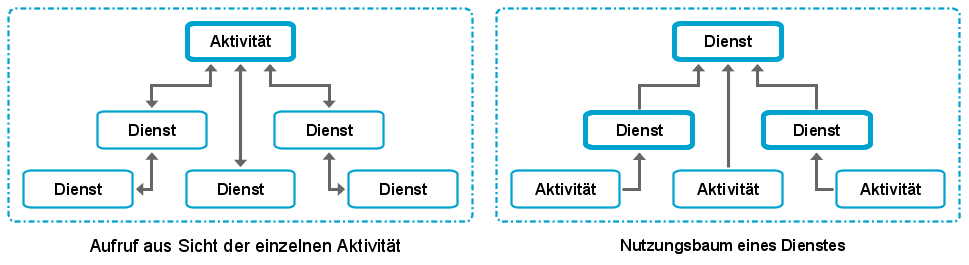
\includegraphics[width=\textwidth]{img/Serviceaufbau.png}	
    \caption[Nutzung eines Dienstes]
    {Nutzung eines Dienstes  \protect\footnotemark}
    \label{fig:Nutzung eines Dienstes}
\end{figure}
\footnotetext{in Anlehnung an \citeauthor{Masak.2007} \citeyear{Masak.2007} \cite{Masak.2007} }

Hierbei wird die wesentliche Geschäftslogik der Aktivitäten in digitalen Diensten gekapselt, während der übergreifende Geschäftsprozess in Form von Anwendungssoftware die eher reaktive und demnach dynamische Ausführungssemantik implementiert. 
\cite{Teusch.2016}
Unter dem Aspekt der Wiederverwendbarkeit eines Dienstes in einer \ac{SOA} sollte des Weiteren der in Abbildung \ref{fig:Nutzung eines Dienstes} illustrierte Umstand, dass digitale Dienste zur Ausführung einer Aktivität auf Basis weiterer Dienste aufgebaut sein können oder im Umkehrschluss ein Dienst von unterschiedlichen Aktivitäten genutzt werden kann, einer kritischen Betrachtung unterzogen werden.
\cite{Masak.2007}

Sogenannte Webservices stellen dabei eine auf \ac{XML} ausgerichtete und auf offenen Standards basierende Technologie zur Realisierung einer \ac{SOA} dar, indem sie die in einer beliebigen Programmiersprache implementierte Geschäftslogik in Form von Diensten anhand vereinheitlichter Schnittstellen nach außen zur Verfügung stellen.
\cite{Masak.2005}
Ein Webservice ist als Maschine-zu-Machine-Kommunikation zu betrachten. Diese Maschinen sprechen über offenen Standards miteinander. 
\cite{Finger.2009b}
Nachdem ein Webservice in ein Anwendungssystem integriert wurde, erfolgt die Kommunikation in der Regel automatisch. 
Ein Endanwender auf der Seite der Benutzerschnittstelle wird nicht zur Kenntnis nehmen, dass die Anwendungssoftware, die er bedient, mit einem Webservice kommuniziert. Dieses Prinzip entspricht ebenfalls dem Grundgedanken einer \ac{SOA}.
\cite{Teusch.2016}
Auf diese Weise können Webservices beispielsweise aus einem Geschäftsprozess heraus aufgerufen werden, ohne ihre konkrete Implementierung zu kennen, was insbesondere in einem geschäftsprozess- oder unternehmensübergreifenden Kontext ein bedeutender Faktor ist. Zur Änderung eines Geschäftsprozesses bedarf es lediglich einer Anpassung der Ausführungssemantik der Anwendungssoftware durch veränderte Aufrufe von bestehenden oder zusätzlichen Webservices. 

\todo{SOA Texte durch SAP Book Quelle ersetzen \cite{Pohl.2009} \cite{Hoppe.2011}}
% \begin{attentionForm}[SOA und Webservices nicht grundsätzlich synonym]
% An dieser Stelle sei jedoch der Hinweis erlaubt, dass das Konzept der Serviceorientierung allgemeiner ist und schon früher existierte als Webservices. Webservices sollten daher nur als eine, wenn auch zum Verfassungszeitpunkt dieses Buches als wahrscheinlich am besten geeignete Möglichkeit zur Realisierung serviceorientierter Architekturen betrachtet werden.
% \end{attentionForm}

Ferner können auch von Menschen ausgeführte Aktivitäten als Dienste gekapselt und mit Benutzerschnittstellen ausgestattet werden, indem die Aufforderung zum Beginn der manuellen Aktivität durch eine geeignete Ausgabe signalisiert wird, woraufhin der erfolgreiche Abschluss der manuellen Aktivität oder ein erforderlicher Abbruch wiederum durch eine Eingabe quittiert wird. 
Auf diese Weise ist auch die Integration manueller Aktivitäten in einen automatisierten Geschäftsprozess möglich.
\cite{Weske.2007}

Für die Konzeption und Implementierung von automatisierbaren Geschäftsprozessen ist eine angemessene Spezifizierung erforderlich, die verschiedene Kriterien erfüllen muss.
Bei der Betrachtung dynamischer Geschäftsprozesse im Rahmen dieser Bachelorarbeit spielen dabei auch solche Merkmale eine herausragende Rolle, welche die Ausprägung dynamischer Eigenschaften anhand einer zielgerichteten Ereignisorientierung und Ereignisverarbeitung unterstützen. 

Im Fokus der Betrachtungen sind verschiedene Kriterien zur Auswahl einer geeigneten Modellierungssprache für das zugrunde liegende Geschäftsprozessmodell von Belang, die in Tabelle \ref{tab:Kriterien für Modellierungssprachen} jeweils mit einer Beschreibung ihrer Bedeutung aufgeführt sind.

\begin{table}[H]
	\centering
	\begin{tabularx}{\textwidth}{l X} 
		\toprule
		\textbf{Kriterium}  &   
		\textbf{Beschreibung}  \\ 
		\toprule
		Funktionalität &   
		Unterstützung verschiedener Aktivitätsarten, die Darstellung sequenzieller, paralleler, alternativer und iterativer Prozessabläufe sowie die Verbindung von Aktivitäten mit Objekten, Relationen und Rollen. \cite{Funk.2010b} \\  \cmidrule(r){1-1} \cmidrule(r){2-2}
		
		Verständlichkeit &   
		Auf fachlicher Modellebene ist eine modellbasierte Darstellung der Geschäftsprozesse erwünscht, die von Fachleuten mit betriebswirtschaftlichem und technischem Hintergrund mit vertretbarem Aufwand verstanden werden kann. \\ \cmidrule(r){1-1} \cmidrule(r){2-2}
		
		Formalisierbarkeit &   
		Die Notation soll formale oder semiformale Modellierungsregeln aufweisen, damit die Konzeption korrekter Geschäftsprozessmodelle unterstützt wird und eine nahtlose Implementierung des technischen Geschäftsprozessmodells erfolgen kann. \cite{Becker.2012}  \\ \cmidrule(r){1-1} \cmidrule(r){2-2}
		
		Unterstützung von \ac{SOA} &   
		Digitale Dienste, insbesondere Webservices, und von Menschen durchgeführte Aktivitäten mit geeigneten Benutzerschnittstellen sollen integriert werden können.  \\ \cmidrule(r){1-1} \cmidrule(r){2-2}
		
		Ereignisverarbeitung &   
		Die Modellierungssprache soll ein Konzept für die Integration von Ereignissen in das Geschäftsprozessmodell enthalten und insgesamt eine hohe Ereignisorientierung aufweisen.   \\ \cmidrule(r){1-1} \cmidrule(r){2-2}
		
		Standardisierung &   
		Die Modellierungssprache soll durch eine zentrale Institution standardisiert worden sein oder zumindest einen anerkannten Industriestandard darstellen. \\ \cmidrule(r){1-1} \cmidrule(r){2-2}
		
		Werkzeugunterstützung &   
		Umfangreiche Softwarewerkzeuge für die Modellierung sollen verfügbar sein.  \\
	    \bottomrule
	\end{tabularx}
	\caption[Kriterien für Modellierungssprachen]
    {Kriterien für Modellierungssprachen für dynamische Geschäftsprozesse}
    \label{tab:Kriterien für Modellierungssprachen}
\end{table}

\subsection{Gegenüberstellung geeigneter Modellierungssprachen}
Im Folgenden werden bekannte und etablierte Modellierungssprachen für die Modellierung von Geschäftsprozessen herangezogen, die als Basis für dynamische Geschäftsprozesse dienen können. 
Diese werden zunächst einzeln begreiflich gemacht und anschließend in Bezug auf die in Tabelle \ref{tab:Kriterien für Modellierungssprachen} genannten Kriterien in einer tabellarischen Übersicht gegenübergestellt. 
% Es ist nicht Ziel des folgenden Abschnitts die \acl{EPK}, \acl{BPMN} 2.0 und  Aktivitätsdiagramme der \acl{UML} ausführlich zu diskutieren und vollumfänglich darzustellen.
Es sollen wesentliche Eigenschaften unds Elemente daraus erklärt werden, die für das Verständnis dieser Bachelorarbeit notwendig sind.

\paragraph{\acl{EPK}}
Die \textit{\acf{EPK}} stellt die zentrale Modellierungssprache in der \acf{ARIS} dar.
Entwickelt wurde die \ac{ARIS}-Architektur bereits \citeyear{Scheer.1991} am Institut für Wirtschaftsinformatik in Zusammenarbeit mit dem \ac{CIM}-Technologie-Transfer-Zentrum an der Universität des Saarlandes in Kooperation mit der SAP AG.\footnote{Am 07. Juli 2014 erfolgte eine Umwandlung der SAP AG von einer Aktiengesellschaft in eine Europäische Aktiengesellschaft (SE).}
\cite{Scheer.1991}
Der Modellierungsansatz der \ac{EPK} hat sich insbesondere im deutschsprachigen Raum als eine der meistverbreitetste semiformale Methode zur Modellierung von Geschäftsprozessen durchgesetzt. 
\cite{Gadatsch.2013}
Diese Verbreitung lässt sich unter anderem darauf zurückzuführen, dass die SAP SE die \ac{EPK} als Standard in ihr Produktportfolio integriert hat. 
\cite{Staud.2006}
In \ac{EPK}s, die nicht sequentiell ablaufen, bilden Konnektoren die Verknüpfungsknoten. Gemeint sind hierbei die aus der Aussagenlogik stammenden konjunktiven, adjunktiven und disjunktiven Verknüfungen. Dadurch wird gewährleistet, dass auch alternative, parallele und iterative Geschäftsprozessabläufe durch logische Ereignisverknüpfungen erstellt werden können.
\cite{Lehmann.2008}

In einer erweiterten \ac{EPK} wird die einfache \ac{EPK}, die sich auf Ereignisse, Funktionen, Prozessschnittstellen, Konnektoren und Kanten beschränkt, um zusätzlich verschiedene Elemente wie die organisatorische Einheit, Informationsobjekte, Anwendungssysteme oder Prozesswegweiser ergänzt. 
\cite{Seidlmeier.2015}
Dadurch ist es möglich umfassende Geschäftsprozessmodelle mit all ihren Beziehungen zum Umfeld des Geschäftsprozesses in semiformaler Form darzustellen, um durch die Modellierungssprache alle Perspektiven auf den Geschäftsprozess miteinander zu verbinden.
\cite{Gadatsch.2013}

\paragraph{\acl{BPMN} 2.0}
Die \textit{\acf{BPMN} 2.0} ist eine weltweit verbreiteter Standard der \ac{OMG} zur Modellierung von Geschäftsprozessen.
Da der ersten Version von \ac{BPMN} kein Metamodell zugrunde liegt, handelt es sich bei \ac{BPMN} in seiner ursprünglichen Gestalt streng genommen nicht um eine Modellierungssprache, dies wurde  mit Version 2.0 jedoch behoben. 
\cite{OMG.2014}

Die \ac{BPMN} 2.0 beinhaltet eine Reihe an Elementen für verschiedene Aktivitäten in einem Geschäftsprozess, wie etwa Sendeaufgaben, Empfangsaufgaben, Benutzeraufgaben, Dienstaufgaben, oder Geschäftsregelaufgaben, und eine Vielzahl an unterschiedlichen Ereignistypen, wie etwa Nachrichten-, Zeit-, Signal- oder Fehlerereignisse. 
Darüber hinaus kann der Ablauf eines Prozesses mithilfe sogenannter Gateways gesteuert werden und es kann zudem auf Datenobjekte zugegriffen werden. 
\cite{Weidlich.2010}
Obwohl die Geschäftsprozessmodellierung in \ac{BPMN} 2.0 bezüglich der konkreten Realisierungstechnologien allgemein gehalten ist, werden \ac{SOA} und Webservices durch die reichhaltige Auswahl an Elementen in besonderem Maße unterstützt.
\cite{Jobst.2010}

\paragraph{Aktivitätsdiagramme der \acl{UML}}
Das Aktivitätsdiagramm ist ein Diagrammtyp, der von der \ac{OMG} sowie der \ac{ISO} zusammen mit anderen Diagrammtypen zur Modellierung von Informationen in der \acf{UML} vereinheitlicht wurde.
\cite{OMG.2014}\cite{ISO.2012}
\ac{UML} ist heute eine der dominiernden Modellierungssprachen zur Darstellung informationstechnischer und anderer Systeme, die sich bereits in vielfältigen Einsatzgebieten in der Praxis bewährt hat.
Neben einer grafischen Notation spezifiziert die \ac{UML} auch die Semantik objektorientierter Komponenten und deren Beziehungen mit definierten Regeln für Strukturen und Abläufe.
\cite{Rumpe.2011}

Obwohl die \ac{UML} ursprünglich nicht für die Modellierung von Geschäftsprozessen entworfen wurde, ist eine Geschäftsprozessmodellierung dennoch durch den Entwurf von Aktivitätsdiagrammen eingeschränkt möglich, da hiermit funktionale Abläufe mit Hilfe von Aktivitäten und Verknüpfungen darstellbar sind. 
\cite{vanRanden.2016}
Wohl aber existieren verschiedene Defizite, etwa bezüglich der Verarbeitung von Ereignissen oder durch eine umständliche Darstellung komplexer Verknüpfungen, da bei der \ac{UML} die Systemorientierung gegenüber der Geschäftsprozessorientierung deutlich prädominiert.
\cite{Staud.2006}

\paragraph{Gegenüberstellung der Modellierungssprachen}
In Tabelle \ref{tab:Bewertung von Modellierungssprachen} wird die Eignung der vorgestellten Modellierungssprachen in Bezug auf die relevanten Kriterien aus dem vorherigen Abschnitt in tabellarischer Form gegenübergestellt.

\newcolumntype{Y}{>{\centering\arraybackslash}X}
\begin{table}[H]
	\centering
	\begin{tabularx}{\textwidth}{l Y Y Y} 
		\toprule
		\textbf{Kriterium}  &   
	    \multicolumn{3}{c}{\textbf{Modellierungssprache}}	  \\   \cmidrule(r){2-4}
	    
	                  &   
		\textbf{\acs{EPK}}\cite{Scheer.1991}\cite{Lehmann.2008}      &
		\textbf{\acs{BPMN}}\cite{OMG.2014}\cite{Weidlich.2010}       &
		\textbf{\acs{UML}}\cite{ISO.2012}\cite{Rumpe.2011}	    \\  \cmidrule(r){1-1} \cmidrule(r){2-2} \cmidrule(r){3-3} \cmidrule(r){4-4}
	    
		Funktionalität &   
		\CIRCLE  &
		\CIRCLE   &
		\CIRCLE		\\ \cmidrule(r){1-1} \cmidrule(r){2-2} \cmidrule(r){3-3} \cmidrule(r){4-4}
		
		Verständlichkeit &   
		\CIRCLE &
		\CIRCLE   &
		\LEFTcircle			\\ \cmidrule(r){1-1} \cmidrule(r){2-2} \cmidrule(r){3-3} \cmidrule(r){4-4}
		
		Formalisierbarkeit &   
		\LEFTcircle	 &
		\CIRCLE   &
		\CIRCLE		\\ \cmidrule(r){1-1} \cmidrule(r){2-2} \cmidrule(r){3-3} \cmidrule(r){4-4}
		
		Unterstützung von \ac{SOA} &   
		\Circle &
		\CIRCLE   &
		\Circle		\\ \cmidrule(r){1-1} \cmidrule(r){2-2} \cmidrule(r){3-3} \cmidrule(r){4-4}
		
		Ereignisverarbeitung &   
		\CIRCLE &
		\CIRCLE   &
		\LEFTcircle	\\ \cmidrule(r){1-1} \cmidrule(r){2-2} \cmidrule(r){3-3} \cmidrule(r){4-4}
		
		Standardisierung &   
		\LEFTcircle	 &
		\CIRCLE   &
		\CIRCLE		\\ \cmidrule(r){1-1} \cmidrule(r){2-2} \cmidrule(r){3-3} \cmidrule(r){4-4}
		
		Werkzeugunterstützung  &
		\CIRCLE &
		\CIRCLE   &
		\CIRCLE		\\ 
	    \bottomrule
	    \multicolumn{4}{c}{
	    Legende:
	    \CIRCLE
	    erfüllt
	    \LEFTcircle
	    bedingt erfüllt
	    \Circle wenig bis nicht erfüllt}
	\end{tabularx}
	\caption[Bewertung von Modellierungssprachen]
    {Bewertung von Modellierungssprachen für dynamische Geschäftsprozesse}
    \label{tab:Bewertung von Modellierungssprachen}
\end{table}

Es wird ersichtlich, dass für die Spezifizierung dynamischer Geschäftsprozessmodelle zwar alle Modellierungssprachen durch Werkzeugunterstützung praktisch anwendbar sind, diese sich allerdings deutlich anhand anderer Kriterien unterscheiden. Auffallend ist des Weiteren, dass die Unterstützung der benötigten Funktionalitäten in allen betrachteten Modellierungssprachen gegeben ist, sodass grundsätzlich die Schlussfolgerung gezogen werden kann, dass alle Modellierungssprachen prinzipiell für die Modellierung dynamischer Geschäftsprozesse einsetzbar sind. 

Aufgrund der zwingenden Ereignisbehandlung des Geschäftsprozessmodells, um für die notwendige Dynamik des Geschäftsprozesses zu sorgen, werden lediglich \ac{EPK} und \ac{BPMN} 2.0 als Modellierungssprachen in Betracht gezogen. 
\ac{BPMN} 2.0 zeichnet sich hierbei durch die erforderliche Untersützung von SOA mit Webservices und eine bessere Ausgestaltung der Ereignisverarbeitung mit umfassenderen Ereigniskonzepten sowie einer unabhängig regulierten Standardisierung aus. Letzteres drückt sich insbesondere in der Möglichkeit der grafischen Modellierung von Geschäftsprozessen und somit einer besseren Modellkonsistenz auf der fachlichen Ebene aus. Aus diesen Gründen fällt die Wahl schließlich auf den Einsatz von \ac{BPMN} 2.0 zur formalen Beschreibung des Geschäftsprozessmodells in Kapitel \ref{ch:Durchfuehrung}. 

\section{Konzept der Ereignisverarbeitung}\label{sec:Ereignisverarbeitung}
In der realen Welt ist eine Wechselwirkung aller Geschehnisse mit einer Vielzahl von divergenten, meist nicht-deterministisch eintretenden Ereignissen zu beobachten, als Konsequenz folgt eine signifikante Beeinflussung auf den Fortgang der Geschehnisse.
\cite{Grauer.2010}
Dieser Tatbestand findet sich auch in den Abläufen und Geschäftsprozessen in Unternehmen wieder.
Ein Unternehmen ist demzufolge gezwungen, auf diese Ereignisse angemessen und möglichst zeitnah zu reagieren – die Unternehmen operieren demnach ereignisgesteuert. 
\cite{Schaaf.2015}
Mit dem Konzept der Ereignisverarbeitung rücken Ereignisse als zentraler Leitgedanke einer Orientierung an Ereignissen in den Fokus der Gestaltung von Geschäftsprozessen, indem Ereignisse als Baustein der Softwarearchitektur und der Geschäftslogik in den Mittelpunkt der Betrachtung rücken. 
\cite{Bruns.2010}

Die resultierenden ereignisgesteuerten Unternehmensanwendungen ermöglichen eine praxisnahe Darstellung der dynamischen Geschäftsprozesse eines Unternehmens. 
Das Ziel ist es dadurch die Agilität, Reaktionsfähigkeit und Echtzeitfähigkeit der Geschäftsprozesse eines Unternehmens zu erhöhen. 
In der Praxis hat eine derartige Ereignisorientierung in Unternehmensanwendungen bereits breiten Zuspruch gefunden. 
\cite{Bruns.2015}
In diesem Kontext beruhen ereignisgesteuerte Architekturen, englisch \ac{EDA}, auf einem ereignisgesteuerten Prinzip, bei dem eine lose Kopplung zwischen den beteiligten Komponenten eines Informationssystems vorgesehen ist.  
In ihrer reinen Ausprägung kommunizieren diese Komponenten ausschließlich mittels sogenannter Ereignisbenachrichtigungen, englisch \textit{Event Messages}, miteinander.
Abbildung \ref{fig:Grundschritte von ereignisgesteuerten Architekturen} illustriert den Ablauf der Grundschritte ereignisgesteuerter Architekturen, deren Charakteristika nachfolgend erläutert werden.
\cite{Schaaf.2015}

\begin{figure}[H]
	\centering 
    \begin{tikzpicture}
        \fill[even odd rule, white] circle (1.5);
    
       \node at (0,0) [
          font  = \sffamily\Large\bfseries\color{black!85},
          align = center
       ]{
          \acs{EDA}
       };
       \arcarrow{197}{ 96}{Erkennen}
       \arcarrow{ 89}{-17}{Verarbeiten}
       \arcarrow{199}{341}{Reagieren}
    \end{tikzpicture}
    \caption[Grundschritte von ereignisgesteuerten Architekturen]
    {Grundschritte von ereignisgesteuerten Architekturen \protect\footnotemark}
    \label{fig:Grundschritte von ereignisgesteuerten Architekturen}
\end{figure}
\footnotetext{in Anlehnung an \citeauthor{Bruns.2010} \citeyear{Bruns.2010} \cite{Bruns.2010} }

Demnach besteht eine zentrale Charakteristik von ereignisgesteuerten Architekturen aus der Komposition von drei Grundschritten: \textit{Erkennen, Verarbeiten und Reagieren von oder auf Ereignisse.}

\paragraph{Erkennen} 
Das Auftreten von relevanten Informationen und Sachverhalten in  den Geschäftsprozessen ist der Ausgangspunkt für die Erkennung von Ereignissen.
Diese Informationen und Sachverhalte werden analysiert, als Ereignisse klassifiziert und spiegeln einen spezifizierten Ausschnitt des Zustands eines Geschäftsprozesses wieder. 
Für registrierte Ereignisse wird ein entsprechendes Ereignisobjekt generiert.
Entscheidend für ereignisgesteuerte Informationssysteme ist, dass die Ereignisse unmittelbar zum Zeitpunkt ihres Auftretens erkannt werden und nicht zeitverzögert.
\cite{Bruns.2010}

\paragraph{Verarbeiten}
Im Verarbeitungsschritt werden die erkannten Ereignisse, die aus unterschiedlichen Ereignisquellen stammen können, analysiert. Bei der Analyse werden Ereignisse zu Einheiten aggregiert, mit anderen Ereignissen verknüft, generalisiert, aufgeteilt oder aber auch als irrelevant eingestuft. 
Gesucht werden Paradigmen in den gesammelten Ereignissen, die bestimmte Beziehungen und Abhängigkeiten zwischen den Ereignissen ausdrücken.
\cite{Hedtstuck.2017}

\paragraph{Reagieren}
Aufgrund von analysierten Mustern, die im Fluss der eingetretenen Ereignisse erkannt wurden, können vielfältige Arten von Reaktionen zeitnah veranlasst werden. 
Die Reaktionen, die angestrebt werden, charkterisieren sich durch Aktualität und Individualität, wie etwa die unmittelbare Übergabe der Ereignisse an Anwendungssysteme, das Senden von Benachrichtigungen, der Aufruf von Funktionen in Form von digitalen Diensten, das Auslösen eines Geschäftsprozesses oder die Initiierung von manuellen Aktivitäten durch menschliche Benutzer, aber auch die Generierung neuer Ereignisse ist eine legitime Reaktion.
\cite{Bruns.2010}

In der Realität existieren allerdings kaum Geschäftsprozesse, bei denen eine ausschließliche Kommunikation mithilfe von Ereignissen und alleinig im Rahmen der beschriebenen Grundschritte einer \ac{EDA} erfolgen, weshalb auch Anwendungen mit teilweiser Ereignisverarbeitung und partieller Anwendung dieser Grundschritte die Umsetzung einer ereignisgesteuerten Architektur zugeschrieben.
\cite{Etzion.2011}
Die \ac{SOA}-Architektur beinhaltet, wie in Abschnitt \ref{sec:Automatisierung} beschrieben, die Konzepte, die notwendig sind, um Echtzeit-Anwendungssysteme zu ermöglichen und die Unterstützung der Dynamik ereignisgesteuerter Geschäftsprozesse zur selben Zeit zu gewährleisten, nicht vollständig.
Eine \ac{SOA} ohne Ereignisverarbeitung ist folglich nicht in der Lage, den aktuellen Zustand von Aktivitäten zu erkennen, da hierzu in Echtzeit temporale und kausale Verbindungen zwischen Geschäftsprozessen und Aktivitäten identifiziert und analysiert werden müssen. 
Eine \ac{EDA} kann als Maßnahme auch eine \ac{SOA} komplementieren, zumal beide Konzepte grundsätzlich modulare und verteilte Informationssysteme mit loser Kopplung unterstützen, um die Vorteile beider Architekturen im Kollektiv zu nutzen. 
Für eine derartige Kombination von \ac{SOA} und \ac{EDA} wird häufig die Bezeichnung Event-Driven SOA genutzt.
In dieser Ausprägung können Ereignisse den Aufruf von digitalen Diensten auslösen, woraufhin im Verlauf, deren Ausführung weitere Ereignisse generiert werden, die parallel von einem Ereignisverarbeitungsdienst analysiert und verarbeitet werden. 
\cite{Bruns.2010}

Im Zusammenhang mit der Ereignisverarbeitung in Unternehmensanwendungen wird der Begriff Echtzeit, englisch real-time, häufig verwendet, um die Aktualität von verarbeiteten Ereignissen zu hervorzuheben.
\cite{Bruns.2015}
Echtzeit wird jedoch nicht im Sinne der Informatik verstanden, wonach für jede Funktion die exakte Einhaltung einer restriktiv vorgeschriebenen Antwortzeit erforderlich ist, um die Gegenwartsbezogenheit und Vorhersagbarkeit von Informationssystemen sicherzustellen.
Vielmehr dominiert ein betriebswirtschaftliches Verständnis, das darauf Bedacht ist, in allen relevanten Informationssystemen aktuelle Informationen bereitzustellen, ohne spezifizierte Leistungskennzahlen zur Erfüllung von Echtzeit zu formulieren.
\cite{Worn.2005}
Unter Echtzeit versteht man aus dieser Sicht daher die möglichst zeitnahe Verfügbarkeit, Transparenz und Nutzbarkeit von Informationen ohne unnötige Zeitverzögerung.
Eingehende Ereignisse werden somit im Rahmen der Ereignisverarbeitung analysiert, sobald sie auftreten, um geeignete Reaktionen in Echtzeit auslösen zu können.
\cite{Grauer.2010}

\subsection{Merkmale und Kriterien}
Die \ac{EDA} wird, wie schon erwähnt, im Wesentlichen durch die drei Grundschritte Erkennen, Verarbeiten und Reagieren charakterisiert, woraus sich drei logische architektonische Schichten für eine Ereignisverarbeitung ergeben: Ereignisquellen, Ereignisverarbeitung und Ereignisbehandlung. Das
Zusammenspiel dieser drei Schichten wird  in Abbildung \ref{fig:Grundlegender architektonischer Entwurf einer EDA} veranschaulicht.

\begin{figure}[H]
	\centering 
    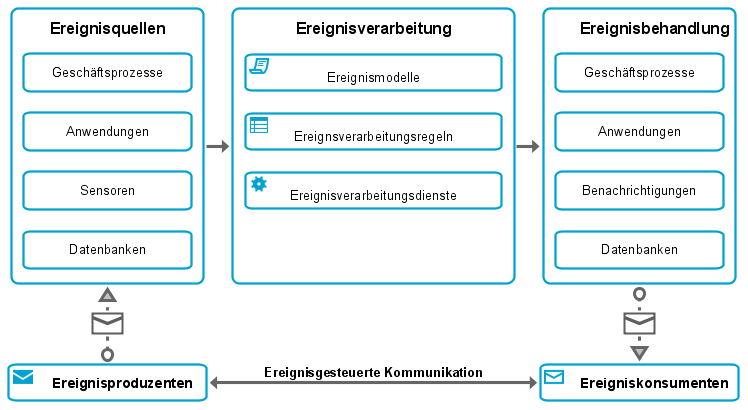
\includegraphics[width=\textwidth]{img/Ereignisverarbitungablauf.png}	
    \caption[Grundlegender architektonischer Entwurf einer EDA]
    {Grundlegender architektonischer Entwurf einer EDA}
    \label{fig:Grundlegender architektonischer Entwurf einer EDA}
\end{figure}
\footnotetext{in Anlehnung an \citeauthor{Metz.2014} \citeyear{Metz.2014} \cite{Metz.2014} }

\todo{abbildung erkären}

\todo{Formulierung der Ereignisverarbeitungsregeln}

\missingfigure{Kriterien für Funktionalitäten der Ereignisverarbeitung}

\subsection{Bewertung von Funktionalitäten der Ereignisverarbeitung}

\todo{Referenzieren auf \cite{Vidackovic.2010}}

\missingfigure{Tabelle  Bewertung von Funktionalitäten der Ereignisverarbeitung}


\section{Dynamische Geschäftsprozesse auf Basis von Ereignisverarbeitung}\label{sec:Kombi}
Bei der Automatisierung von dynamischen Geschäftsprozessen wächst die Notwendigkeit, auf kritische Ereignisse in Echtzeit und ohne Latenzzeiten zu reagieren. 
Die Integration von Ereignisverarbeitungskonzepten in die Konzeption dynamischer Geschäftsprozesse ist ein geeignetes Mittel, um den steigenden Anforderungen an das Echtzeit-Management von Geschäftsprozessen unter Berücksichtigung relevanter Ereignisse zur Laufzeit gerecht zu werden. 
\cite{Abolhassan.2016}
Die Vorteile für ein Unternehmen bei einer solchen Vervollständigung der Geschäftsprozessautomatisierung mit Konzepten der Ereignisverarbeitung gründen sich im Wesentlichen auf die folgenden Merkmale:

\begin{itemize}
    \item 
    Identifizierung relevanter oder kritischer Situationen für den Geschäftsprozess unter Berücksichtigung externer Ereignisse aus dem Geschäftsumfeld und interner Ereignisse aus dem Geschäftsprozess.
    \item 
    Möglichkeit der unmittelbaren Reaktion auf veränderliche Situationen durch Verarbeitung von Ereignissen in Echtzeit.
    \item
    Möglichkeit der Trennung der Ereignisverarbeitungslogik von der Geschäftsprozesslogik durch lose Kopplung und Kommunikation über Ereignisobjekte.Automatisierte Adaptionen von Geschäftsprozessen auf Basis von aktuellen Ereignissen.
    \item
    Gute Unterstützung von verteilten Umgebungen, die insbesondere in unternehmensübergreifenden Geschäftsprozessnetzwerken und \ac{SOA}-Umgebungen eine bedeutende Rolle spielen.
\end{itemize}

Es existieren bereits erste Forschungsansätze mit dem Ziel der Anreicherung von Geschäftsprozessmodellen mit Konzepten der Ereignisverarbeitung, die unter der englischen Bezeichnung Event-Driven Business Process Management zusammengefasst werden. Ausgewählte Konzepte aus diesem Bereich werden im Folgenden vorgestellt und anschließend anhand wesentlicher Kriterien gegenübergestellt.

\subsection{Merkmale und Kriterien}

Dynamische und somit ereignisorientierte Geschäftsprozesse operieren prinzipiell auf zwei Ebenen, der Geschäftsprozessebene und der Ereignisverarbeitungsebene. 
Diese erfüllen ihre Aufgaben in erster Linie separat und in paralleler Weise, kommunizieren allerdings mittels des Austauschs von Ereignissen miteinander, was in diesem Kontext den maßgeblichen Aspekt darstellt. 
Abbildung \ref{fig:Ebenen dynamischer Geschäftsprozesse} illustriert in schematischer Darstellung die Zusammenhänge.

\begin{figure}[H]
	\centering 
    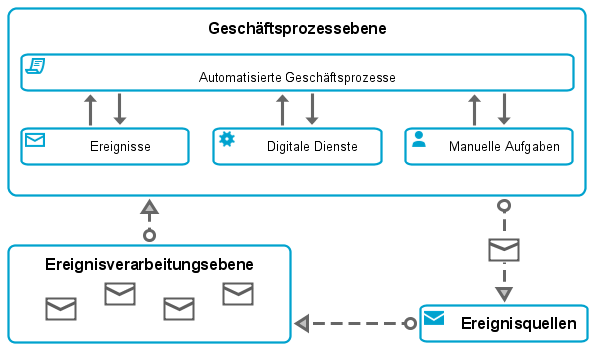
\includegraphics[width=\textwidth]{img/dynamicbp.png}	
    \caption[Ebenen dynamischer Geschäftsprozesse]
    {Ebenen dynamischer Geschäftsprozesse \protect\footnotemark}
    \label{fig:Ebenen dynamischer Geschäftsprozesse}
\end{figure}
\footnotetext{Eigene Darstellung, in Anlehnung an \citeauthor{Vidackovic.2014} \citeyear{Vidackovic.2014} \cite{Vidackovic.2014} }
\footnotetext{Die Abbildung dient lediglich der Visualisierung und ist nicht \ac{BPMN} 2.0 konform.}

Auf der Ereignisverarbeitungsebene werden eingehende Ereignisse aus diversen externen und internen Ereignisquellen kontinuierlich analysiert, wobei zudem Ereignisse generiert werden können, welche wiederum dieselbe Analyse durchlaufen. 
Da zwischen der Ereignisverarbeitungsebene und der Geschäftsprozessebene mit Ereignissen kommuniziert werden kann, können diese generierten Ereignisse als unmittelbare Reaktion eine dynamische Wirkung auf den Ablauf des laufenden Geschäftsprozess ausüben.
Der Geschäftsprozess fungiert demnach einerseits als eine der internen Ereignisquellen für die Ereignisverarbeitungsebene und andererseits als wesentlicher Ereigniskonsument der generierten Ereignisse zur Adaption des Prozessablaufs.
\cite{Benker.2016}

Auf der Geschäftsprozessebene erfolgt der operative und automatisierte Ablauf von Aktivitäten des Geschäftsprozesses, wobei Letztere in einer \ac{SOA} überwiegend auf elektronischen Diensten basieren, die als Webservices über standardisierte Schnittstellen aufgerufen werden und auch über Unternehmensgrenzen hinweg verteilt sein können.
\cite{Finger.2009}
Bei den Aktivitäten kann es sich darüber hinaus auch um manuelle Benutzeraufgaben handeln, die zwar von Menschen ausgeführt werden, aber dennoch mittels informationstechnischen Schnittstellen in einen automatisierten Prozessablauf integriert werden können.
\cite{Bruns.2010}


In ereignisorientierten im Gegensatz zu ablauforientierten Geschäftsprozessen üben Ereignisse zur Laufzeit einen signifikanten Einfluss auf den Prozessablauf aus, sodass die Geschäftsprozesse anhand geeigneter Ereignisverarbeitungsregeln mit dynamischen Eigenschaften ausgestattet werden können. 

\subsection{Gegenüberstellung vorhandener Forschungsansätze}
Die wesentlichen Aspekte der existierenden Forschungsansätze werden zunächst einzeln betrachtet und anschließend gegenübergestellt.

\paragraph{Entwicklung agiler Geschäftsprozesse mit Ereignisverarbeitung}
Dieser Forschungsansatz von \citeauthor{Alexopoulou.2008} aus dem Jahr \citeyear{Alexopoulou.2008} liefert eine Vorgehensweise zur Entwicklung dynamischer und ereignisgesteuerter Geschäftsprozesse, die nicht in Form eines abgeschlossenen Systems modelliert werden, sondern lediglich aus einzelnen Ereignis-Aktivität-Einheiten, sogenannten Dynamikeinheiten, bestehen. 
\cite{Alexopoulou.2008} 
Diese werden in Echtzeit auf der Ereignisverabreitungsebene ausgeführt und fügen den Geschäftsprozess dynamisch zusammen, wobei neue Ereignis-Aktivität-Einheiten bedarfsgerecht hinzugefügt werden können. 

Ein Defizit dieses Forschungsansatzes ist die fehlende Betrachtung des gesamten Ablaufs. Das Konzept dieser Dynamikeinheiten wird auch in dieser Bachelorarbeiten aufgegriffen, allerdings ausgehend von einem in seiner Gesamtheit modellierten Geschäftsprozess, der in diese Einheiten zerlegt wird.

\paragraph{RESTful SOA zur Automatisierung von Geschäftsprozessen}
Die Realisierung von \ac{SOA} in diesem Forschungsansatz von \citeauthor{Wolf.2016} ist in Übereinstimmung mit den Prinzipien von \ac{REST}. 
\footnote{
Da der technische Fokus in dieser Arbeit auf der Geschäftsprozessebene liegt, werden die einzelnen technischen Konzepte an dieser Stelle nicht weiter vertieft.
Für eine detaillierte Betrachtung der Prinzipien von \ac{REST} sei lediglich auf weiterführende Literatur verwiesen.
\cite{Wolf.2016}\cite{Masak.2007}\cite{Finger.2009}}
Die \ac{REST}ful \ac{SOA} entsteht durch den Entwurf serviceorientierter Architekturen gemäß den Bedingungen und Technologien von \ac{REST}. \ac{REST} ist ein Architekturstil für die Gestaltung verteilter Systeme, insbesondere bei der Umsetzung von Webservices. Durch dieses Vorgehen wird auf eine modellbasierte Spezifikation von \ac{REST}ful \ac{SOA} für die Automatisierung von Geschäftsprozessen abgezielt. \cite{Wolf.2016}

Insbesondere die Überwindung der semantischen Lücke zwischen Geschäftsprozessmodell und Anwendungssystem durch ein systematisches Vorgehen wird in diesem Forschungsansatz behandelt. Die identifizierten Probleme werden durch einen Ansatz zur Konzeption eines Anwendungssystems auf Basis von auf fachlicher Ebene modellierten Geschäftsprozessen angegangen.  
Es fehlen allerdings Möglichkeiten zur Modellierung wesentlicher Konzepte der Echtzeitverarbeitung von Ereignissen.
Da der Forschungsansatz wohl aber auf die automatisierte Ausführung von Geschäftsprozessen mithilfe von digitalen Diensten ausgerichtet ist, bleibt der Ansatz für die softwaretechnische Implementierung in Kapitel von Relevanz. 

\paragraph{Methodology for Business Dynamics\textsuperscript{dbpm}}
Der Forschungsansatz von \citeauthor{Vidackovic.2014} stellt die  Methode [moby]\textsuperscript{dbpm} zur Entwicklung dynamischer Geschäftsprozesse mit Ereignisverarbeitung dar. Der Name [moby]\textsuperscript{dbpm} steht dabei für Methodology for Business Dynamics und dbpm für Dynamic Business Process Management. Der Ansatz bietet einen geeigneten Lösungsansatz für die Problemstellung dynamischer Geschäftsprozesse mit Ereignisverabeitung an und stellt das dafür benötigte, webbasierte Modellierungswerkzeug zur Verfügung. 
\cite{Vidackovic.2014}

Die Modellierung wird in einer von \citeauthor{Vidackovic.2014} erweiterten Form von \ac{BPMN} 2.0 vorgenommen. Des Weiteren folgt der Ansatz den Konzepten der modellbasierten Softwarentwicklung. Die Geschäftsprozessmodelle können in Kombination mit dem Produkt \textit{Esper} mit Code angereichert und anschließend automatisch ausgeführt werden ohne eine weitere Implementierung in ein Anwendungssystem. Der Ansatz einer modellbasierten Softwarentwicklung wird im Rahmen dieser Bachelorarbeit, aufgrund mangelnder Integrationsmöglichkeiten mit SAP S/4HANA Cloud, nicht weiter verfolgt. Die Ergebnisse des Forschungsansatzes von \citeauthor{Vidackovic.2014} werden jedoch als wertvoller Beitrag in diesem Fachbereich angesehen.  

\paragraph{SOEDA-Methode}
SOEDA beschreibt ein Verfahren zur Entwicklung von Anwendungssystemen durch die Zusammenführung von serviceorientierten (SOA) und ereignisgesteuerten Architekturen (EDA). Geschäftsprozesse werden hier mit \ac{EPK}s modelliert. 
\cite{MatthiasWieland.2009} 
Mit Hilfe von grafischen Modellierungswerkzeugen werden die zugrunde liegenden Aktivitäten modularisiert und mit entsprechenden Ereignissen gekoppelt, so dass ein Entwickler die Regeln der Ereignisverarbeitung anschließend in einer spezifischen Programmiersprache implementieren kann. 
\cite{Bruns.2010}

Schwächen der SOEDA-Methode sind die unzureichende Modellierung von Ereignisverarbeitungsregeln durch die Verwendung von \ac{EPK}s. 
\cite{RobraBissantz.2009}
Auch mangelt es an der Abbildung von Ereignissen im Geschäftsprozess, da Ereignisse nur als Teil des normalen Geschäftsprozessablaufs betrachtet werden. Mit der Version 2.0 verfügt die \ac{BPMN}, wie in Abschnitt \ref{sec:Automatisierung} erwähnt, nun nicht nur über eine grafische Notation, sondern auch über die Semantik der technischen Ausführung. Auf \ac{EPK}s kann demzufolge im Rahmen der Bachelorarbeit verzichtet werden, zumal eine Konsistenz des Geschäftsprozessmodells auf betriebswirtschaftlicher und technischer Ebene wünschenswert ist.

\paragraph{Gegenüberstellung der Ansätze}
Auf Basis der Darstellung der existierenden Forschungsansätze wird ersichtlich, dass die bestehenden Forschungsansätze für die Anreicherung von Geschäftsprozessmodellen mit Konzepten der Ereignisverarbeitung jeweils einen bestimmten Fokus besitzen, dessen Herausforderungen im Einzelfall ausreichend erfüllt werden. 
Eine Kopplung von Ereignissen und Aktivitäten mithilfe des Ansatzes von \citeauthor{Alexopoulou.2008}, fachliche Aspekte wie die der SOEDA-Methode, die technischen Möglichkeiten der \enquote{RESTful SOA} oder eine automatisierte Ausführung der [moby]\textsuperscript{dbpm} finden beispielsweise keine Betrachtung. 

Folglich lässt sich sagen, dass bisher noch kein Lösungsansatz mit einer ganzheitlichen und durchgängigen Vorgehensweise existiert, die eine vollständige, formale sowie fachlich orientierte Modellierung von Geschäftsprozessen mit dynamischen Eigenschaften auf Basis von Ereignisverarbeitung ermöglicht.


\section{Zusammenfassung der wesentlichen Erkenntnisse und Defizite}


\todo{Anpassen}

Resümierend sind im Wesentlichen folgende Erkenntnisse festzuhalten, die für die betrachtete Pro-
blemstellung von Relevanz sind:
\begin{itemize}
	\item This is a bullet point.
    \item This is another one.
\end{itemize}

Diesen Erkenntnissen kann durch den aktuellen Stand der Wissenschaft und Technik nicht in
reichendem Maße Rechnung getragen werden, da maßgebliche Defizite vorhanden sind:
\begin{itemize}
	\item This is a bullet point.
    \item This is another one.
\end{itemize}